\documentclass[a4paper,utf8]{article}
\usepackage{ctex}
\usepackage{blindtext}
\usepackage[utf8]{inputenc}
\usepackage{amsmath,bm}
\usepackage{amstext}
\usepackage{amsfonts}
\usepackage{amsmath}
\usepackage{epsfig}
\usepackage[colorlinks,linkcolor=blue]{hyperref}
\usepackage{setspace}
%图片     
\usepackage{subfigure}         
\usepackage{natbib}
\usepackage{float}
\usepackage{epstopdf}
\usepackage{graphicx}

\title{Introduction to Machine Learning\\Homework 3}
\author{181860155 朱晓晴\\\href{mailto:heloize@126.com}{heloize@126.com}}

\begin{document}
	\maketitle
	\numberwithin{equation}{section}
	
	\section{[20pts] Decision Tree}

	\noindent (1) [10pts] Assume there is a space contains three binary features $X$, $Y$, $Z$ and the objective function is $f(x,y,z)=\neg(x \text{ XOR } y)$. Let $H$ denotes the decision tree constructed by these three features. Please answer the following question:
	\begin{itemize}
		\item Is function $f$ realizable? 
		\item If the answer is yes, please draw the decision tree $H$ otherwise please give the reason.\\
	\end{itemize}
	(2) [10pts] Consider the following matrix:
	$$
	\left[
	\begin{matrix}
	24 & 53 & 23 & 25 & 32 & 52 & 22 & 43 & 52 & 48 \\
	40 & 52 & 25 & 77 & 48 & 110 & 38 & 44 & 27 & 65\\
	\end{matrix}
	\right]
	$$
	which contains 10 examples and each example contains two features $x_1$ and $x_2$. The corresponding label of these 10 examples as follows:
	$$
	\left[
	\begin{matrix}
	1 & 0 & 0 &1 & 1 & 1 & 1& 0 & 0 & 1
	\end{matrix}
	\right]
	$$
	In this problem, we want to build a decision tree to do the classification task.
	\begin{itemize}
		\item Calculate the entropy of the root node.
		\item Building your decision tree. What is your split rule  and the classification error?\\
	\end{itemize}
	解:
	(1) $f$可实现,决策树如下图所示:
	\begin{figure}[H]
		\centering
		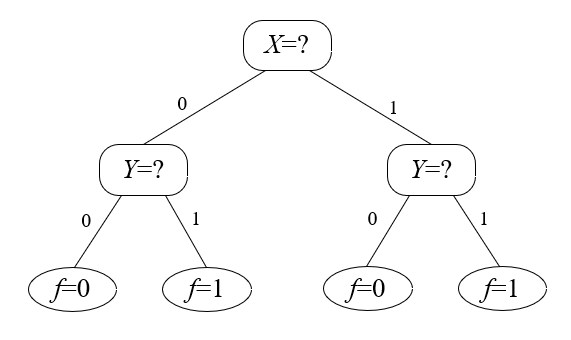
\includegraphics[scale=0.7]{p1-dt1.PNG}
		\caption{基于函数$f$生成的决策树}
	\end{figure}

	\noindent (2) 根结点的信息熵为
	\begin{align*}
		\text{Ent}(D)=-\sum\limits_{k=1}^2 p_k log_2 p_k
		=-(\frac{4}{10}log_2\frac{4}{10}+\frac{6}{10}log_2\frac{6}{10})
		=0.97095
	\end{align*}

	对属性$x_1$,将样本中$x_1$的取值从小到大排序,将$\frac{x_1^i+x_1^{i+1}}{2}$作为侯选划分点,得到
	\begin{align*}
		T_{x_1}=\{22.5,23.5,24.5,28.5,37.5,45.5,50,52,52.5\}
	\end{align*}
	依次计算
	\begin{align*}
		\text{Gain}(D,x_1,x_1^i)
		=\text{Ent}(D)-\sum\limits_{v=1}^2\frac{|D^v|}{|D|}\text{Ent}(D^v)
	\end{align*}
	得到
	\begin{align*}
		& \text{Gain}(D,x_1,22.5)=0.07898,\text{Gain}(D,x_1,23.5)=0.00740,\text{Gain}(D,x_1,24.5)=0.00580 \\
		& \text{Gain}(D,x_1,28.5)=0.04644,\text{Gain}(D,x_1,37.5)=0.12451,\text{Gain}(D,x_1,45.5)=0.01997 \\
		& \text{Gain}(D,x_1,50)=0.09128,\text{Gain}(D,x_1,52)=0.00740,\text{Gain}(D,x_1,52.5)=0.14448
	\end{align*}
	$x_1$信息增益为0.14448,对应划分点52.5。

	对属性$x2$,有
	\begin{align*}
		T_{x_2}=\{26,32.5,39,42,46,50,58.5,71,93.5\}
	\end{align*}
	\begin{align*}
		& \text{Gain}(D,x_1,26)=0.14448,\text{Gain}(D,x_1,32.5)=0.32193,\text{Gain}(D,x_1,39)=0.09128 \\
		& \text{Gain}(D,x_1,42)=0.019973,\text{Gain}(D,x_1,46)=0.12451,\text{Gain}(D,x_1,50)=0.04644 \\
		& \text{Gain}(D,x_1,58.5)=0.28129,\text{Gain}(D,x_1,71)=0.17095,\text{Gain}(D,x_1,93.5)=0.07898
	\end{align*}
	$x_2$信息增益为0.32193,对应划分点32.5。
	因此,以$x_2$为根节点划分属性。

	对于下一层的左结点,划分出的样本标记都为0,无需继续划分。
	对于右结点,可按照上述计算出
	$x_1$信息增益为0.31128,对应划分点37.5;
	$x_2$信息增益为0.20443,对应划分点58.5。
	因此,以$x_1$为该节点划分属性。

	对于下一层的左结点,划分出的样本标记都为1,无需继续划分。
	对于右结点,可按照上述计算出
	$x_1$信息增益为0.31128,对应划分点45.5和52.5;
	$x_2$信息增益为1,对应划分点58.5。
	因此,以$x_2$为该节点划分属性。

	对于下一层的左结点,划分出的样本标记都为0,无需继续划分。
	对于右结点,划分出的样本标记都为1,无需继续划分。

	决策树如下图所示:
	\begin{figure}[H]
		\centering
		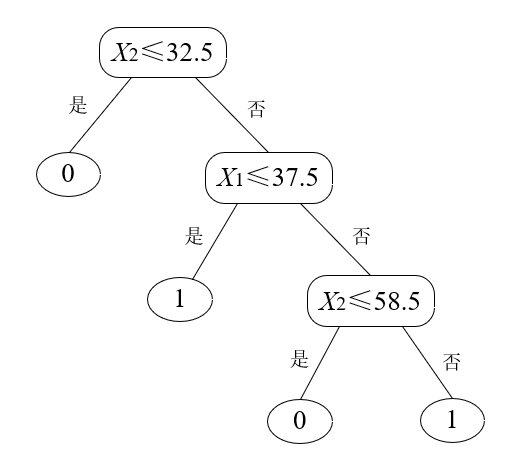
\includegraphics[scale=0.7]{p1-dt2.PNG}
		\caption{基于信息增益生成的决策树}
	\end{figure}

	该决策树的分类误差为0。
	



	\newpage
	\section{[20pts] Neural Network}
	\noindent Consider the following neural network, consisting of two input units, a single hidden layer containing two units, and one output unit:
	
	\begin{figure}[htbp]
		\centering
		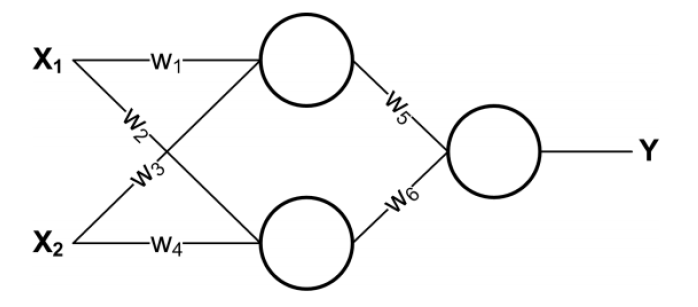
\includegraphics[scale=0.5]{p2-nn1.png}
		\caption{神经网络}
	\end{figure}

	(1) [5pts] Assume that the network is using linear units: that is, for a given unit $U$, $A$ is the vector of activations of units that send their output to $U$ and $W$ is the weight vector corresponding to these outputs, then the output of the unit is $W^{\mathrm{T}}A$. Let the weight values $w_i$ be fixed, re-design the neural network to compute the same function without using any hidden units. Express the new weights in terms of the old weights.
	
	(2) [5pts] Is it always possible to express a neural network made up of only linear units without a hidden layer?
	
	(3) [10pts] Choose an activation function for each unit in the network which will cause this network to learn the same function that logistic regression would learn. Each unit should use a logistic, linear, or threshold activation function, with no constraints on the weights.
	\\
	
	\noindent 解:
	(1) 新的神经网络如下图所示:
	\begin{figure}[htbp]
		\centering
		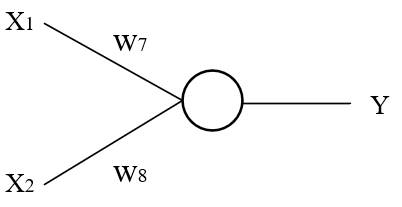
\includegraphics[scale=0.7]{p2-nn2.png}
		\caption{仅使用线性单元的神经网络}
	\end{figure}
	
	\noindent 其中$w_7=w_1w_5+w_2w_6$,$w_8=w_3w_5+w_4w_6$。

	\noindent (2) 
	总是能以没有隐藏层的形式表示一个仅由线性单元构成的神经网络。
	因为由线性单元构成的神经网络的输出总是能够用矩阵乘法表示,
	以题中的神经网络为例,输出可以表示为:
	\begin{align*}
		& Y=w_5(w_1x_1+w_3x_2)+w_6(w_2x_1+w_4x_2) \\
		& =(w_1w_5+w_2w_6)x_1+(w_3w_5+w_4w_6)x_2 \\
		& =\left[
			\begin{matrix}
				w_5 & w_6
			\end{matrix}
			\right] 
			\left[
			\begin{matrix}
				w_1 & w_3 \\
				w_2 & w_4
			\end{matrix}
			\right]
			\left[
			\begin{matrix}
				x_1 \\
				x_2
			\end{matrix}
			\right]
	\end{align*}
	因此,如果网络有$n$个输入,分别为$x_1,x_2,\dots ,x_n$,
	输出可以表示为:
	\begin{align*}
		Y=B_mB_{m-1}\dots B_1
		\left[
		\begin{matrix}
			x_1 & x_2 & \dots & x_n
		\end{matrix}
		\right]^{\mathrm{T}}
	\end{align*}
	其中$B_j$为每一层的权重构成的矩阵。
	那么,将各个输入$x_i$直接与输出层神经元相连,
	令其权重为$B_mB_{m-1}\dots B_1$乘积中第$i$列元素的值,
	即可得到符合题意的不含隐藏层的神经网络。

	\noindent (3) 
	令隐藏层上下两个神经元分别为$E$和$F$,输出层神经元为$G$。\\
	$E$的激活函数为$f_1(x)=x$,
	输出为$f_1(W_1^{\mathrm{T}}A)=w_1x_1+w_3x_2$,
	其中
	$$
		W_1=\left[
		\begin{matrix}
			w_1 \\
			w_3
		\end{matrix}	
		\right], 
		A=\left[
		\begin{matrix}
			x_1 \\
			x_2
		\end{matrix}	
		\right]
	$$
	$F$的激活函数为$f_2(x)=x$,
	输出为$f_2(W_2^{\mathrm{T}}A)=w_2x_1+w_4x_2$,
	其中
	$$
		W_1=\left[
		\begin{matrix}
			w_2 \\
			w_4
		\end{matrix}	
		\right]
	$$
	$G$的激活函数为$f_3(x)=(1+e^{-x})^{-1}$,
	输出为
	$$
	f_3(W_3^{\mathrm{T}}A_1)=(1+e^{-(w_1w_5+w_2w_6)x_1+(w_3w_5+w_4w_6)x_2})^{-1}
	$$
	其中
	$$
		W_3=\left[
		\begin{matrix}
			w_5 \\
			w_6
		\end{matrix}	
		\right], 
		A_1=\left[
		\begin{matrix}
			w_1x_1+w_3x_2 \\
			w_2x_1+w_4x_2
		\end{matrix}	
		\right]
		=\left[
		\begin{matrix}
			W_1^{\mathrm{T}} \\
			W_2^{\mathrm{T}}
		\end{matrix}	
		\right]A
	$$





	\newpage
	\section{[60 pts] Neural Network in Practice}
	
	\noindent In this task, you are asked to build a Convolutional Neural Networks (CNNs) from scratch and examine performance of the network you just build on \textbf{MNIST} dataset.
	Fortunately, there are some out-of-the-box deep learning tools that can help you get started very quickly. For this task, we would like to ask you to work with the \textbf{Pytorch} deep learning framework. Additionally, Pytorch comes with a built-in dataset class for MNIST digit classification task in the \textbf{torchvision} package, including a training set and a validation set. You may find a pytorch introduction at \href{https://pytorch.org/tutorials/beginner/blitz/cifar10_tutorial.html}{here}. Note that, you can use CPU or GPU for training at your choice.
	
	Please find the detailed requirements below.\\

	(1) [5 pts] You are encouraged to implement the code using \emph{Python3}, implementations in any other programming language will not be judged. Please name the source file (which contains the main function) as \emph{CNN\underline{\hspace{0.5em}}main.py}. Finally, your code needs to print the performance on the provided validation set once executed.

	(2) [20 pts] Use any type of CNNs as you want and draw graphs to show your network architecture in the submitted report. You are encouraged to try more architectures.

	(3) [25 pts] During training, you may want to try some different optimization algorithms, such as SGD, Adam. Also, you need to study the effect of learning rate and the number of epoch, on the performance (accuracy).
		    
	(4) [10 pts] Plot graphs (learning curves) to demonstrate the change of training loss as well as the validation loss during training.


	\newpage
	\section*{实验报告}
	\subsection*{1 实验环境}
	本次实验的环境如下:

	Python 3.8.3
	
	PyTorch 1.7.0
	
	CUDA 11.0


	\subsection*{2 卷积神经网络}
	本次实验采用了Gradient-Based Learning Applied to Document Recognition
	提出的LeNet-5卷积神经网络,其结构如下图所示:
	\begin{figure}[H]
		\centering
		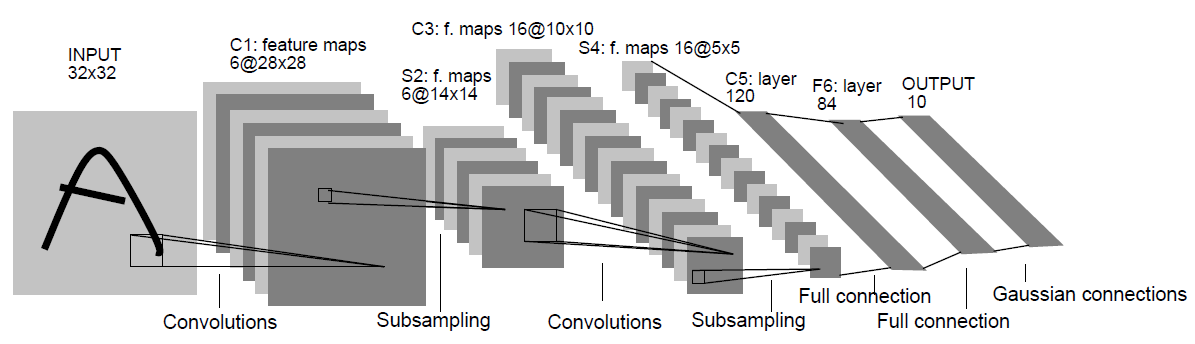
\includegraphics[scale=0.6]{p3-lenet5.PNG}
		\caption{LeNet-5结构}
	\end{figure}

	由于MNSIT数据集提供的样本数据以$28\times 28\times 1$的形式组织,
	因此需要对LeNet-5结构进行调整,调整后的结构如下:

	输入:$28\times 28\times 1$的图像

	C1:卷积层,使用6个$3\times 3$的滤波器,步长为1,padding采用Same方式,输出$28\times 28\times 6$的图像。

	S2:池化层,使用$2\times 2$的滤波器,步长为2,输出$14\times 14\times 6$的图像。

	C3:卷积层,使用16个$3\times 3$的滤波器,步长为1,padding采用Valid方式,输出$10\times 10\times 16$的图像。

	S4:池化层,使用$2\times 2$的滤波器,步长为2,输出$5\times 5\times 16$的图像。

	C5和F6:全连接层,分别有120个和84个神经元。

	输出层:10个神经元


	\subsection*{3 代码实现}
	基于上一节中的理论,本次实验设计了如下数据结构和模块划分:

	LeNet5类:用于构建LeNet-5卷积神经网络,卷积层和全连接层使用ReLu作为激活函数,代码实现见图6。

	Train函数:通过学习60000个样本来训练CNN。

	Test函数:用训练出的CNN测试10000个样本
	\begin{figure}[H]
		\centering
		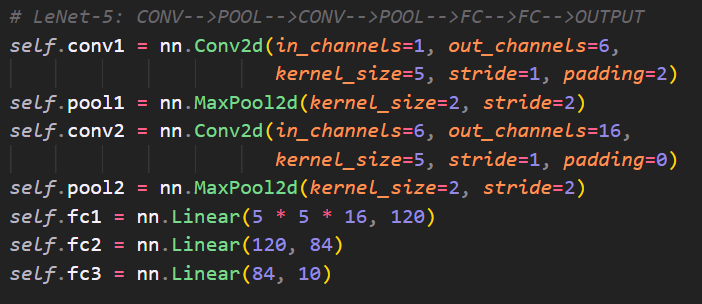
\includegraphics[scale=0.8]{p3-lenet5-code.PNG}
		\caption{LeNet-5代码实现}
	\end{figure}

	代码的执行流程大致如下:

	1.读取MNIST训练集和测试集。

	2.定义LeNet5类,并创建CNN实体net。

	3.确定损失函数和优化算法。

	4.训练卷积神经网络。

	5.测试并输出CNN的性能数据。


	\subsection*{4 参数选取}
	实验鼓励尝试不同的优化算法和超参数,
	本节将对以上2个方面进行讨论,并选出相对更优的配置。
	激活函数和损失函数则采用神经网络中常见的ReLU和交叉熵损失。

	\subsubsection*{4.1 优化算法}
	给定以下参数
	\begin{align*}
		& \text{LR=0.01} \\
		& \text{BATCH\underline{\hspace{0.5em}}SIZE=50}
	\end{align*}
	分别使用SGD和Adam优化算法训练模型,得到的测试准确率如下表所示:
	\begin{table}[h]
		\centering
		\label{tab:my_label}
		\begin{tabular}{|c|c|c|c|}
		   \hline
		   Accuracy & epoch=1 & epoch=2 & epoch=5 \\
		   \hline
		   SGD & 97.66\% & 98.22\% & 98.90\% \\
		   \hline
		   Adam & 97.81\% & 97.61\% & 97.90\% \\
		   \hline
		\end{tabular}
		\caption{使用SGD和Adam优化的准确率}
	\end{table}

	根据上表数据,易知在LeNet-5结构下,
	SGD优化算法的表现较Adam优化算法更好。
	同时,根据traning loss和validation loss的图像(未给出),
	采用Adam算法进行优化时,模型更易、更早出现过拟合。
	因此,本次实验选用SGD作为优化算法,算法参数momentum=0.9。


	\subsubsection*{4.2 超参数}
	采用LeNet-5结构,令BATCH\underline{\hspace{0.5em}}SIZE=50,
	对不同的学习率和epoch进行研究,得到的测试准确率如下表所示:
	\begin{table}[h]
		\centering
		\label{tab:my_label}
		\begin{tabular}{|c|c|c|c|c|c|c|}
		   \hline
		   Accuracy & epoch=1 & epoch=2 & epoch=3 & epoch=4 & epoch=5 & epoch=8 \\
		   \hline
		   lr=0.005 & 96.70\% & 97.86\% & 98.20\% & 98.51\% & 98.53\% & 98.72\% \\
		   \hline
		   lr=0.01  & 97.66\% & 98.22\% & 98.82\% & 98.91\% & 98.90\% & 98.84\% \\
		   \hline
		   lr=0.02 & 97.82\% & 98.05\% & 98.73\% & 98.44\% & 98.87\% & 99.04\% \\
		   \hline
		   lr=0.05 & 98.07\% & 98.42\% & 97.82\% & 98.62\% & 98.24\% & 98.75\% \\
		   \hline
		\end{tabular}
		\caption{不同学习率和epoch下的准确率}
	\end{table}

	根据上表中的数据,易发现当学习率一定时,准确率基本随着epoch的增大而增大。
	考虑到epoch越大时,准确率增加得越缓慢,本次实验选用的参数为
	\begin{align*}
		& \text{LR=0.01} \\
		& \text{EPOCH=5} \\
		& \text{BATCH\underline{\hspace{0.5em}}SIZE=50}
	\end{align*}


	\subsection*{5 实验结果}
	由第4节的讨论结果,本次实验最终采用LeNet-5结构、SGD优化算法和以下参数,
	并在本节给出训练出的模型的性能指标。
	\begin{align*}
		& \text{LR=0.01} \\
		& \text{EPOCH=5} \\
		& \text{BATCH\underline{\hspace{0.5em}}SIZE=50}
	\end{align*}

	模型在10000个样本的MNIST数据集上的准确率为98.90\%(见表2)。
	
	训练时,
	每学习完1个mini-batch(即50个样本),会输出这个batch的训练损失。
	同时,会选取测试集中的100个样本,由当前模型进行预测,得到验证损失。
	最终,得到如下的training loss和validation loss曲线。
	\begin{figure}[H]
		\centering
		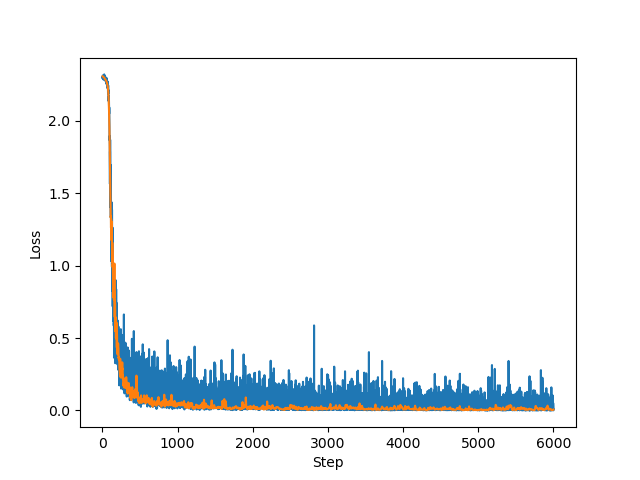
\includegraphics[scale=0.7]{p3-learning-curves.PNG}
		\caption{学习曲线}
	\end{figure}

\begin{thebibliography}{1}
\bibitem{ref1} 周志华. 机器学习[M]. 清华大学出版社, 2016.
\bibitem{ref2} 卷积神经网络\\\url{https://www.jianshu.com/p/c0215d26d20a}
\bibitem{ref3} 常见卷积神经网络\\\url{https://www.cnblogs.com/guoyaohua/p/8534077.html}
\bibitem{ref4}	LeNet-5实现MNIST分类(Tensorflow2实现)\\\url{https://www.cnblogs.com/nickhan-cs/p/13340869.html}
\bibitem{ref5} 随机梯度下降算法\\\url{https://blog.csdn.net/qq_38150441/article/details/80533891}
\bibitem{ref6} cifar10\underline{\hspace{0.5em}}tutorial\\\url{https://pytorch.org/tutorials/beginner/blitz/cifar10_tutorial.html}
\bibitem{ref7} 根据损失曲线诊断神经网络\\\url{https://blog.csdn.net/sjwzdh/article/details/103523465}
\end{thebibliography}


\end{document}